% Options for packages loaded elsewhere
% Options for packages loaded elsewhere
\PassOptionsToPackage{unicode}{hyperref}
\PassOptionsToPackage{hyphens}{url}
\PassOptionsToPackage{dvipsnames,svgnames,x11names}{xcolor}
%
\documentclass[
  nonatbib,
  authoryear,
  preprint]{elsarticle}
\usepackage{xcolor}
\usepackage{amsmath,amssymb}
\setcounter{secnumdepth}{5}
\usepackage{iftex}
\ifPDFTeX
  \usepackage[T1]{fontenc}
  \usepackage[utf8]{inputenc}
  \usepackage{textcomp} % provide euro and other symbols
\else % if luatex or xetex
  \usepackage{unicode-math} % this also loads fontspec
  \defaultfontfeatures{Scale=MatchLowercase}
  \defaultfontfeatures[\rmfamily]{Ligatures=TeX,Scale=1}
\fi
\usepackage{lmodern}
\ifPDFTeX\else
  % xetex/luatex font selection
\fi
% Use upquote if available, for straight quotes in verbatim environments
\IfFileExists{upquote.sty}{\usepackage{upquote}}{}
\IfFileExists{microtype.sty}{% use microtype if available
  \usepackage[]{microtype}
  \UseMicrotypeSet[protrusion]{basicmath} % disable protrusion for tt fonts
}{}
\makeatletter
\@ifundefined{KOMAClassName}{% if non-KOMA class
  \IfFileExists{parskip.sty}{%
    \usepackage{parskip}
  }{% else
    \setlength{\parindent}{0pt}
    \setlength{\parskip}{6pt plus 2pt minus 1pt}}
}{% if KOMA class
  \KOMAoptions{parskip=half}}
\makeatother
% Make \paragraph and \subparagraph free-standing
\makeatletter
\ifx\paragraph\undefined\else
  \let\oldparagraph\paragraph
  \renewcommand{\paragraph}{
    \@ifstar
      \xxxParagraphStar
      \xxxParagraphNoStar
  }
  \newcommand{\xxxParagraphStar}[1]{\oldparagraph*{#1}\mbox{}}
  \newcommand{\xxxParagraphNoStar}[1]{\oldparagraph{#1}\mbox{}}
\fi
\ifx\subparagraph\undefined\else
  \let\oldsubparagraph\subparagraph
  \renewcommand{\subparagraph}{
    \@ifstar
      \xxxSubParagraphStar
      \xxxSubParagraphNoStar
  }
  \newcommand{\xxxSubParagraphStar}[1]{\oldsubparagraph*{#1}\mbox{}}
  \newcommand{\xxxSubParagraphNoStar}[1]{\oldsubparagraph{#1}\mbox{}}
\fi
\makeatother


\usepackage{longtable,booktabs,array}
\usepackage{calc} % for calculating minipage widths
% Correct order of tables after \paragraph or \subparagraph
\usepackage{etoolbox}
\makeatletter
\patchcmd\longtable{\par}{\if@noskipsec\mbox{}\fi\par}{}{}
\makeatother
% Allow footnotes in longtable head/foot
\IfFileExists{footnotehyper.sty}{\usepackage{footnotehyper}}{\usepackage{footnote}}
\makesavenoteenv{longtable}
\usepackage{graphicx}
\makeatletter
\newsavebox\pandoc@box
\newcommand*\pandocbounded[1]{% scales image to fit in text height/width
  \sbox\pandoc@box{#1}%
  \Gscale@div\@tempa{\textheight}{\dimexpr\ht\pandoc@box+\dp\pandoc@box\relax}%
  \Gscale@div\@tempb{\linewidth}{\wd\pandoc@box}%
  \ifdim\@tempb\p@<\@tempa\p@\let\@tempa\@tempb\fi% select the smaller of both
  \ifdim\@tempa\p@<\p@\scalebox{\@tempa}{\usebox\pandoc@box}%
  \else\usebox{\pandoc@box}%
  \fi%
}
% Set default figure placement to htbp
\def\fps@figure{htbp}
\makeatother


% definitions for citeproc citations
\NewDocumentCommand\citeproctext{}{}
\NewDocumentCommand\citeproc{mm}{%
  \begingroup\def\citeproctext{#2}\cite{#1}\endgroup}
\makeatletter
 % allow citations to break across lines
 \let\@cite@ofmt\@firstofone
 % avoid brackets around text for \cite:
 \def\@biblabel#1{}
 \def\@cite#1#2{{#1\if@tempswa , #2\fi}}
\makeatother
\newlength{\cslhangindent}
\setlength{\cslhangindent}{1.5em}
\newlength{\csllabelwidth}
\setlength{\csllabelwidth}{3em}
\newenvironment{CSLReferences}[2] % #1 hanging-indent, #2 entry-spacing
 {\begin{list}{}{%
  \setlength{\itemindent}{0pt}
  \setlength{\leftmargin}{0pt}
  \setlength{\parsep}{0pt}
  % turn on hanging indent if param 1 is 1
  \ifodd #1
   \setlength{\leftmargin}{\cslhangindent}
   \setlength{\itemindent}{-1\cslhangindent}
  \fi
  % set entry spacing
  \setlength{\itemsep}{#2\baselineskip}}}
 {\end{list}}
\usepackage{calc}
\newcommand{\CSLBlock}[1]{\hfill\break\parbox[t]{\linewidth}{\strut\ignorespaces#1\strut}}
\newcommand{\CSLLeftMargin}[1]{\parbox[t]{\csllabelwidth}{\strut#1\strut}}
\newcommand{\CSLRightInline}[1]{\parbox[t]{\linewidth - \csllabelwidth}{\strut#1\strut}}
\newcommand{\CSLIndent}[1]{\hspace{\cslhangindent}#1}



\setlength{\emergencystretch}{3em} % prevent overfull lines

\providecommand{\tightlist}{%
  \setlength{\itemsep}{0pt}\setlength{\parskip}{0pt}}



 


\usepackage{booktabs}
\usepackage{longtable}
\usepackage{array}
\usepackage{multirow}
\usepackage{wrapfig}
\usepackage{float}
\usepackage{colortbl}
\usepackage{pdflscape}
\usepackage{tabularx}
\usepackage{xltabular}
\usepackage{threeparttable}
\usepackage{threeparttablex}
\usepackage[normalem]{ulem}
\usepackage{makecell}
\usepackage{xcolor}
\usepackage{threeparttable}
\usepackage{pdflscape}
\usepackage{unicode-math}
\usepackage[margin=4cm]{geometry}
\usepackage{etoolbox}
\AtBeginEnvironment{longtable}{\footnotesize}
\AtBeginEnvironment{tabular}{\small}
\AtBeginDocument{\setlength{\parindent}{2\parindent}}
\makeatletter
\@ifpackageloaded{caption}{}{\usepackage{caption}}
\AtBeginDocument{%
\ifdefined\contentsname
  \renewcommand*\contentsname{Table of contents}
\else
  \newcommand\contentsname{Table of contents}
\fi
\ifdefined\listfigurename
  \renewcommand*\listfigurename{List of Figures}
\else
  \newcommand\listfigurename{List of Figures}
\fi
\ifdefined\listtablename
  \renewcommand*\listtablename{List of Tables}
\else
  \newcommand\listtablename{List of Tables}
\fi
\ifdefined\figurename
  \renewcommand*\figurename{Figure}
\else
  \newcommand\figurename{Figure}
\fi
\ifdefined\tablename
  \renewcommand*\tablename{Table}
\else
  \newcommand\tablename{Table}
\fi
}
\@ifpackageloaded{float}{}{\usepackage{float}}
\floatstyle{ruled}
\@ifundefined{c@chapter}{\newfloat{codelisting}{h}{lop}}{\newfloat{codelisting}{h}{lop}[chapter]}
\floatname{codelisting}{Listing}
\newcommand*\listoflistings{\listof{codelisting}{List of Listings}}
\makeatother
\makeatletter
\makeatother
\makeatletter
\@ifpackageloaded{caption}{}{\usepackage{caption}}
\@ifpackageloaded{subcaption}{}{\usepackage{subcaption}}
\makeatother
\journal{psyarxiv}
\usepackage{bookmark}
\IfFileExists{xurl.sty}{\usepackage{xurl}}{} % add URL line breaks if available
\urlstyle{same}
\hypersetup{
  pdftitle={Very little data tampering is needed to manufacture statistically significant results: A Monte Carlo simulation study},
  pdfauthor={Ian Hussey},
  colorlinks=true,
  linkcolor={blue},
  filecolor={Maroon},
  citecolor={Blue},
  urlcolor={Blue},
  pdfcreator={LaTeX via pandoc}}


\setlength{\parindent}{6pt}
\begin{document}

\begin{frontmatter}
\title{Very little data tampering is needed to manufacture statistically
significant results:\\
A Monte Carlo simulation study}
\author[1]{Ian Hussey%
\corref{cor1}%
}
 \ead{ian.hussey@unibe.ch} 

\affiliation[1]{organization={University of Bern},,postcodesep={}}

\cortext[cor1]{Corresponding author}

        
\begin{abstract}
Fabricating a statistically significant result does not require
fabricating a dataset. I simulate a dishonest analyst who starts from
data generated under the true null hypothesis and alters, deletes, or
invents one data point at a time, always the point that most helps,
re-running the test after every change until \emph{p} \textless{} .05. I
formalize this as a family of iterative algorithmically-greedy tampering
strategies (dropping cases, switching condition labels, re-pairing
values, duplicating cases, fabricating cases, and replacing cases)
across three common designs: the two-group mean difference (Student's
t-test), the Pearson correlation, and the 2x2 association (chi-square
test). Each strategy runs until significance is reached or further
tampering becomes structurally impossible, and the estimand is the
effort required: the number of tampered data points, both absolutely and
as a proportion of the sample. Two findings recur. First, effort is
small in absolute terms and falls steeply in relative terms as samples
grow. Median tamper counts rise only slowly with sample size, from a
handful of data points at N = 20 to a few dozen at N = 400, so expressed
as a share of the sample the effort drops by roughly an order of
magnitude. Large studies are therefore proportionally easier to corrupt,
not safer. Second, the strategy that is hardest to detect in the
two-group design, because it leaves every univariate distribution
untouched (condition switching), is also among the cheapest; its
correlation analogue (value re-pairing) is cheaper than duplication and
costs about as much as unprincipled case deletion, while being invisible
to any check of either variable alone. I conclude that fabrication and
falsification of results typically requires a worryingly small amount of
actual data tampering.
\end{abstract}





\end{frontmatter}
    

\section{Introduction}\label{introduction}

In November 2019, the pivotal trial of a treatment for ANCA-associated
vasculitis was unblinded and its primary analysis run. The result was
not significant (\emph{p} = .1025). According to a subsequent letter
from the US Food and Drug Administration, unblinded personnel employed
by the sponsor then selected nine of the trial's 331 patients for
re-adjudication of their remission status, having first confirmed that
reclassifying five of them would move the study across the significance
threshold. The five were reclassified, the database was re-locked, and
the re-run analysis returned \emph{p} = .0132. That analysis was the
only one submitted in support of approval, which was granted in 2021. In
April 2026 the FDA proposed to withdraw it, concluding that the
integrity of the trial had been compromised; the sponsor contests this
and a hearing is pending
(\citeproc{ref-us_food_and_drug_administration_center_for_drug_evaluation_and_research_proposal_2026}{U.S.
Food and Drug Administration, Center for Drug Evaluation and Research,
2026}). Whatever its resolution, one feature of the case is worth
dwelling on. Five records out of 331, just 1.5\% of the sample,
separated a failed trial from a successful one.

How often does it occur that data are simply tampered with until
statistical significance is reached? Meta-analysis of the survey
literature puts self-admitted research misconduct at 2.9\% of
researchers (95\% CI {[}2.1, 3.8{]}), comprising 1.9\% for fabrication
and 3.3\% for falsification, while 15.5\% report having witnessed it in
others (\citeproc{ref-xie_prevalence_2021}{Xie et al., 2021}; see also
\citeproc{ref-fanelli_how_2009}{Fanelli, 2009}). When the National
Survey on Research Integrity used a randomized response design to give
respondents provable deniability, admitted fabrication rose to 4.3\% and
falsification to 4.2\%
(\citeproc{ref-gopalakrishna_prevalence_2022}{Gopalakrishna et al.,
2022}). From the other side of the desk, 24\% of consulting
biostatisticians in a US national survey had been asked, at least once
in the preceding five years, to remove or alter data records to better
support a research hypothesis (\citeproc{ref-wang_researcher_2018}{Wang
et al., 2018}). These are not the rates of a vanishing phenomenon, and
each is likely a lower bound of the true prevalence.

Prevalence, though, is only half the question. The other half is how
`effective' such data manipulations actually are. Here, the literature
is largely silent. Chambers (\citeproc{ref-chambers_seven_2017}{2017})
set out a ``dirty dozen'' of ways to guarantee significant results even
under the null hypothesis, the second of which is switching participants
between conditions. Brown (\citeproc{ref-brown_condition_2020}{2020})
posted a short simulation of the efficacy of this in a blog post. Both
convey the same intuition that a handful of unjustified changes to the
data is enough to produce statistically significant results in many
cases, but neither is a systematic assessment. The field has no
systematic account of how much tampering a given strategy requires,
whether that requirement grows with sample size, how the strategies
compare with one another, or how large an effect they leave behind.

For the ambiguous end of the continuum of merely `questionable' research
practices, that gap has been filled. Stefan \& Schönbrodt
(\citeproc{ref-stefan_big_2023}{2023}) compiled 12 \emph{p}-hacking
strategies from the literature, identified the factors controlling each
one's severity, and simulated the resulting increase in false-positive
rates. Their scope, as they state it, is the ``grey area between good
practice and outright scientific misconduct''. They stop deliberately at
its far edge: discussing misreported test statistics, they note that at
some point one must ask whether a practice is still questionable or has
become outright fraud. As such, the literature says comparably little
about the impact of indefensible research practices on false-positive
rates. Of course, given a willingness to engage in an arbitrary amount
of data falsification or fabrication, by definition one can obtain
statistically significant results. Here, I ask a narrower question: how
much data tampering, of what form, is typically needed to acquire
significant results.

Quantifying the indefensible practices is worth doing because of how
researchers appear to decide what to do. Entradas et al.
(\citeproc{ref-entradas_shades_2026}{2026}) find that perceived
seriousness is by far the strongest predictor of whether a researcher
engages in a questionable practice, ahead of every career and
demographic factor they measure. Equally, in John et al.
(\citeproc{ref-john_measuring_2012}{2012}), deciding whether to exclude
data after seeing its effect on the results was admitted by 38--43\% of
psychologists and rated 1.61 out of 2 for defensibility, while
falsifying data was admitted by 0.6--1.7\% and rated 0.16. These results
are consistent with the idea of perceived norms shaping research
behaviors. That is, if researchers are more likely to engage in
practices they understand to be seriously problematic and are less
likely to engage in ones that are seen as such. However, the boundary
between these plausibly varies between individuals, research
communities, and over time, creating what is effectively an Overton
Window of questionable versus unacceptable research practices. Many
research practices that were regarded as acceptable prior to the
invention of the term \emph{p}-hacking are now considered in many
research communities to be substantially less acceptable. If perceptions
of how problematic a given set of research behaviors are influence the
prevalence of those behaviours, then establishing how relatively bad a
given set of practices actually are, how little effort they take, and
how much bias they inject, likely represents important information to
dissuading their practice.

This perspective is an explicitly social-epistemological one, which
understands researcher behaviors as a set of evolving community norms
rather than moral acts. Equally, this perspective is concerned only with
the undesirable statistical consequences of certain researcher
behaviors, but is agnostic to researchers' intent when taking them. With
that being said, at a human level, it is easier to imagine a researcher
who deletes a small number of data points to `reveal' an effect they
strongly believe is there, lying just under the surface of the data,
when it is not (e.g., cases of `qualitative exclusion strategies':
Schiller et al. (\citeproc{ref-schiller_addendum_2018}{2018})) than to
imagine scientists simply making up datasets wholesale {[}although the
latter does occur; Verfaellie \& McGwin
(\citeproc{ref-verfaellie_case_2011}{2011}){]}, despite both strategies
producing false-positive results. Regardless of whether these two
scenarios can be equated in their intent, it is an open question whether
they can be equated in their outcomes, as it is generally unclear how
relatively robust or fragile most results are to modifications of only a
small number of data points (although see
\citeproc{ref-spiess_scientific_2024}{Spiess et al., 2024}).

Some definition matters are worth considering, insofar as they informed
which tampering strategies were simulated. The US government's Office of
Research Integrity provides influential definitions of research
misconduct and its forms
(\citeproc{ref-steneck_introduction_2007}{Steneck, 2007}). According to
the ORI definitions, fabrication is ``making up data or results and
recording or reporting them''. This is represented by the the
fabrication, duplication and replacement strategies simulated here,
which add data points. Falsification is ``manipulating research
materials, equipment, or processes, or changing or omitting data or
results such that the research is not accurately represented in the
research record''. This is represented by the dropping strategy (which
omits observations) and the condition switching and re-pairing
strategies (which change labels and pairings without adding or deleting
anything). The taxonomy that carries the regulatory and moral weight
thus classifies by mechanism: was the data point invented, or was it
altered or omitted? Of course, the line is not necessarily clear here,
given that an altered data point is equivalent to a removed data point
plus a newly added data point.

In this article I do three things. First, I formalize data tampering as
a family of iterative greedy algorithms (dropping, condition switching,
re-pairing, duplication, fabrication, and replacement) applied to three
of the most common elementary designs: the two-group mean difference
(Student's \emph{t}-test), the Pearson correlation, and the 2×2
association (chi-square test). Second, I estimate the effort each
strategy requires, with the full design specified under the ADEMP
framework (\citeproc{ref-morris_using_2019}{Morris et al., 2019};
\citeproc{ref-siepe_simulation_2024}{Siepe et al., 2024}) and every
estimate accompanied by a Monte Carlo standard error. I invert the
design used in previous simulations to understand the impact of
\emph{p}-hacking. Where Stefan \& Schönbrodt
(\citeproc{ref-stefan_big_2023}{2023}) fix a budget of manipulations and
measure the resulting false-positive rate, I fix the goal (statistical
significance) and measure the number of tampered data points required to
reach it. I take this to be the more ecologically valid framing for
deliberate tampering: an analyst who has decided to manufacture a result
does not set a budget in advance and stop when it is exhausted, but
continues until the \emph{p}-value crosses. It also yields effort
directly, in units of edited data points. Because the simulations run
without any tampering budget, the complete distribution of required
effort is observed, and the proportion of datasets exceeding any given
budget is recovered afterwards from the same runs. Third, I show that
the effort required is small, that it does not grow with sample size in
proportional terms, and that the strategies hardest to detect are among
the cheapest.

\section{Methods}\label{methods}

The design is specified under the ADEMP framework (Aims, Data-generating
processes, Estimands, Methods, Performance measures)
(\citeproc{ref-morris_using_2019}{Morris et al., 2019}), as
operationalized for psychology by Siepe et al.
(\citeproc{ref-siepe_simulation_2024}{2024}). The three research
compendia containing all simulation code, per-strategy results, and
extended rationale are available in the project repository (see
\emph{Data and code availability}); this section compresses them.

\subsection{Aims}\label{aims}

The study is descriptive: there is no closed-form benchmark for the
minimum number of tampered points needed to manufacture significance,
because that number is a property of a tampering algorithm applied to
random data, not an estimator of a population parameter. For each
strategy and sample size I aim to estimate (1) how many tampered data
points are required to first reach \emph{p} \textless{} .05, absolutely
and as a proportion of the sample, and how this scales with sample size;
(2) the proportion of datasets requiring more than a given share of the
sample (post hoc budgets of 10\% and 25\%), and the proportion for which
significance is never attained at all; and (3) how the strategies
compare on these measures.

\subsection{Data-generating processes}\label{data-generating-processes}

All data are generated under the true null, so every significant result
is a false positive produced entirely by the tampering.

\begin{itemize}
\tightlist
\item
  Mean difference. Two independent groups of \texttt{n\_per\_condition}
  observations each, \(Y_{ij} \sim \mathcal{N}(\mu_j, \sigma^2)\) with
  \(\mu_{\text{control}} = \mu_{\text{intervention}} = 0\) and
  \(\sigma = 1\).
\item
  Correlation. A bivariate Normal sample of \(n\) observations with
  \(\rho = 0\) and unit variances.
\item
  2×2 association. Two groups (exposed, not exposed) of
  \texttt{n\_per\_condition} observations with a binary outcome drawn at
  the same Bernoulli prevalence in both groups; prevalence is varied
  (.20 vs .05) to contrast a common with a rare outcome.
\end{itemize}

Per-group sample sizes are 10 and 25 to 200 in steps of 25 (total \(N\)
= 20--400; the correlation setting uses the same total \(N\)s). Fully
crossing strategy with sample size (and prevalence) gives 45 conditions
in each continuous setting and 54 in the binary setting, each replicated
10,000 times.

\subsection{Estimands}\label{estimands}

The estimand is \texttt{tampers\_needed}: the number of tampering
operations applied before the test first returns \emph{p} \textless{}
.05, reported both as a count and as a proportion of the sample. The
compendia also record the effect size of each final tampered dataset,
but those are not analysed here: this article is concerned with the
effort required to manufacture a false positive rather than with the
size of the effect that results.

\subsection{Methods (tampering
strategies)}\label{methods-tampering-strategies}

Every strategy is an iterative greedy procedure: generate a null
dataset, test it, and while non-significant, apply one tampering
operation targeting the data point most opposed to the desired result,
then re-test. Table~\ref{tbl-strategies} defines the operations. All
strategies push toward a positive effect by convention; tests are
two-sided at \(\alpha = .05\) (equal-variance \emph{t}-test; Pearson
correlation test; chi-square test without continuity correction).

\begin{longtable}[]{@{}
  >{\raggedright\arraybackslash}p{(\linewidth - 6\tabcolsep) * \real{0.2159}}
  >{\raggedright\arraybackslash}p{(\linewidth - 6\tabcolsep) * \real{0.2614}}
  >{\raggedright\arraybackslash}p{(\linewidth - 6\tabcolsep) * \real{0.2614}}
  >{\raggedright\arraybackslash}p{(\linewidth - 6\tabcolsep) * \real{0.2614}}@{}}
\caption{The tampering strategies and their operationalization in each
setting. Each operation counts as one tampered data point. For binary
data, duplication, fabrication, and replacement collapse onto the same
atomic operation (adding a favourable cell) and are treated as a single
strategy.}\label{tbl-strategies}\tabularnewline
\toprule\noalign{}
\begin{minipage}[b]{\linewidth}\raggedright
Strategy
\end{minipage} & \begin{minipage}[b]{\linewidth}\raggedright
Mean difference
\end{minipage} & \begin{minipage}[b]{\linewidth}\raggedright
Correlation
\end{minipage} & \begin{minipage}[b]{\linewidth}\raggedright
2×2 association
\end{minipage} \\
\midrule\noalign{}
\endfirsthead
\toprule\noalign{}
\begin{minipage}[b]{\linewidth}\raggedright
Strategy
\end{minipage} & \begin{minipage}[b]{\linewidth}\raggedright
Mean difference
\end{minipage} & \begin{minipage}[b]{\linewidth}\raggedright
Correlation
\end{minipage} & \begin{minipage}[b]{\linewidth}\raggedright
2×2 association
\end{minipage} \\
\midrule\noalign{}
\endhead
\bottomrule\noalign{}
\endlastfoot
Dropping & Delete the most hostile case (lowest in intervention or
highest in control) & Delete the most discordant case (most negative
centred cross-product) & Delete a 1 from not-exposed or a 0 from
exposed \\
Label switching & Move the most hostile case's \emph{condition label} to
the other group, alternating direction to keep groups balanced &
\emph{Re-pairing:} swap the \emph{y}-values of two cases so the most
discordant case receives the \emph{y} matching its \emph{x}-rank & Move
a not-exposed 1 to exposed or an exposed 0 to not-exposed, alternating
direction \\
Duplication & Duplicate a case from each group's most favourable 10\% &
Duplicate one of the most concordant cases & (coincides with
fabrication) \\
Fabrication & Add invented cases: control \(\sim \mathcal{N}(0, 0.2)\),
intervention \(\sim \mathcal{N}(5, 0.2)\) & Add a high-leverage
concordant pair at \(\pm(3, 3)\) with small scatter & Add a 1 to exposed
or a 0 to not-exposed \\
Replacement & Replace the most hostile case with an invented one
(whichever of the two candidate replacements most lowers \emph{p}) &
Replace the most discordant case's \emph{y} with a concordant
high-leverage value & (coincides with fabrication) \\
\end{longtable}

The label-switching column deserves emphasis because of its forensic
properties: condition switching leaves every univariate distribution
untouched, and re-pairing preserves both marginal distributions
\emph{exactly} (the set of \emph{y}-values is only permuted), so neither
is detectable by any univariate check. Swapping \emph{entire}
conditions, as opposed to individual cases, is handled analytically
rather than simulated: it merely doubles the directional false-positive
rate to \(\alpha\), adding \(\tfrac{1}{2}\alpha\).

No tampering budget is imposed. Each strategy runs until significance is
reached or a structural limit is hit, such removing all datat under
dropping. A loop guard is included at 10× the sample size as a
termination backstop (e.g., a one-step greedy cannot cross the two-sided
test's \(p \approx 1\) valley when the initial dataset happens to show a
strong effect in the \emph{opposite} direction; such iterations, well
under 1\% of runs, are recorded as never attaining significance).
Because the full unbudgeted counts are recorded, the proportion of
datasets exceeding \emph{any} tampering budget is computable after the
fact; I report budgets of 10\% and 25\% of the sample.

\subsection{Performance measures and Monte Carlo
uncertainty}\label{performance-measures-and-monte-carlo-uncertainty}

An iteration that never attains significance has no finite tamper count
(i.e., is right-censored). All percentile-based summaries (median, 95\%
prediction interval) are therefore computed over all iterations with the
never-significant ones ranked above every finite count; a percentile
falling among them is reported as \emph{never} rather than being
silently replaced by the survivors' percentile, which would answer a
different question (``given that tampering worked, how many edits?'')
and bias the effort downward. The mean cannot be computed this way at
all (the censored counts are unbounded above), so means are reported
only as conditional-on-success skew diagnostics. Two intervals are used.
The interquartile range is plotted, because one condition (correlation
duplication at the smallest sample size) has a 97.5th percentile at
nearly nine times the sample and would otherwise set the scale for every
panel. The 95\% prediction interval is reported in
Table~\ref{tbl-results}. Effort as a proportion is expressed relative to
the \emph{original} sample size, so strategies that append cases, or
re-tamper a case already tampered with, can exceed 1.

Every reported estimate carries a Monte Carlo standard error: binomial
for proportions, closed-form for means, and nonparametric bootstrap for
medians (\citeproc{ref-morris_using_2019}{Morris et al., 2019};
\citeproc{ref-siepe_simulation_2024}{Siepe et al., 2024}). In tables,
decimal places are set from the MCSE (two significant figures, with the
estimate rounded to match) rather than fixed per table. Simulations were
parallelized with reproducible L'Ecuyer--CMRG streams, so results are
identical regardless of worker count.

\section{Results}\label{results}

\begin{figure}

\centering{

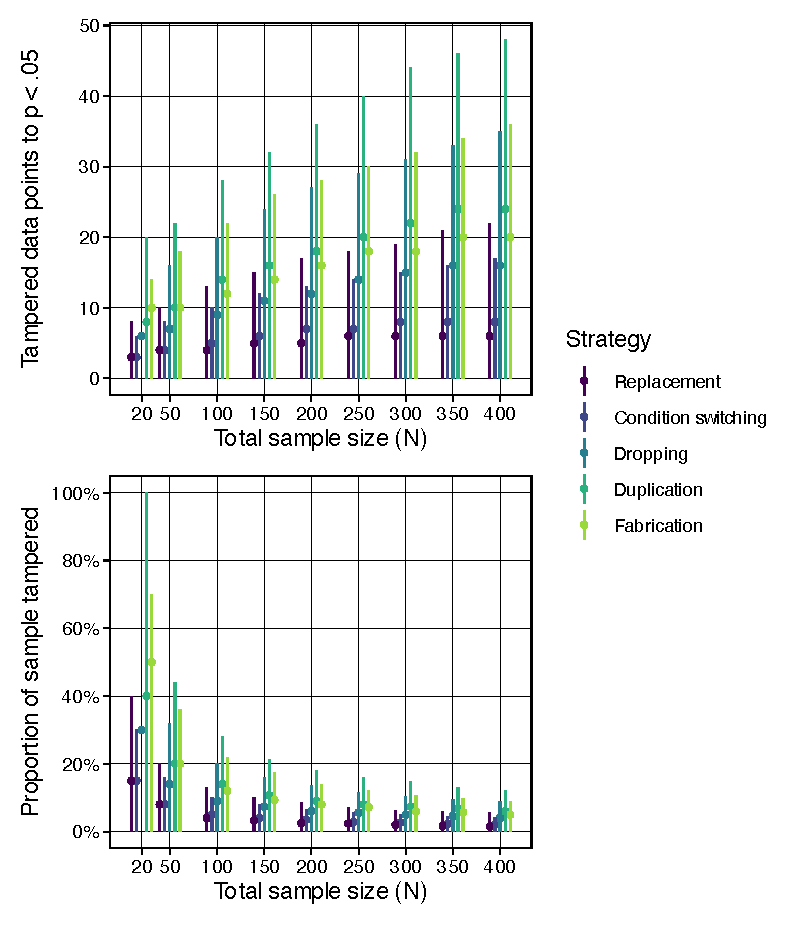
\includegraphics[width=1\linewidth,height=\textheight,keepaspectratio]{manuscript_files/figure-pdf/fig-meandiff-1.pdf}

}

\caption{\label{fig-meandiff}Mean-difference (t-test) setting: the
number of tampered data points needed to first reach p \textless{} .05
(top) and the same effort as a proportion of the sample (bottom). Points
are censoring-aware medians and bars are interquartile ranges. A bar
ending in a hollow triangle is open-ended: more than a quarter of those
datasets never attained significance, so the upper quartile has no
finite value and the bar is drawn to the top of the data range. The
lower panel expresses effort relative to the \emph{original} sample
size, so strategies that append cases or re-tamper the same case can
exceed 1. Strategies are ordered by median proportion tampered. K =
10,000 iterations per condition.}

\end{figure}%

\begin{figure}

\centering{

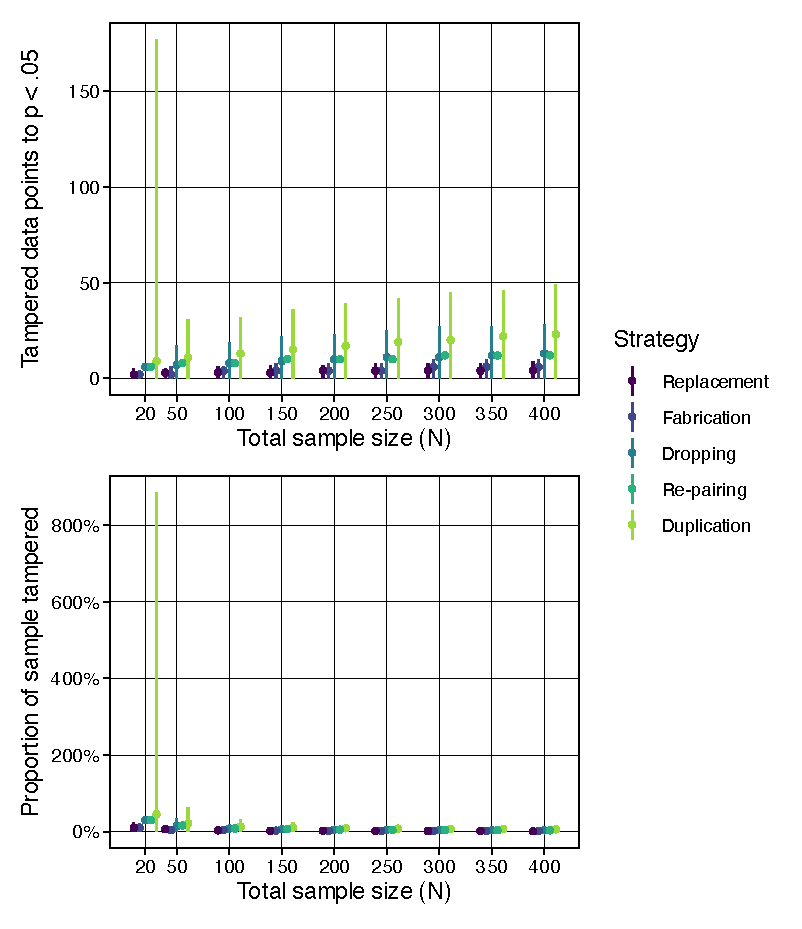
\includegraphics[width=1\linewidth,height=\textheight,keepaspectratio]{manuscript_files/figure-pdf/fig-correlation-1.pdf}

}

\caption{\label{fig-correlation}Correlation setting: tampered data
points needed to first reach p \textless{} .05 (top) and as a proportion
of the sample (bottom). Points are censoring-aware medians and bars are
interquartile ranges; a bar ending in a hollow triangle is open-ended,
its upper quartile falling among datasets that never attained
significance. Effort in the lower panel is relative to the
\emph{original} sample size, so strategies that append cases can exceed
1. K = 10,000 iterations per condition.}

\end{figure}%

\begin{figure}

\centering{

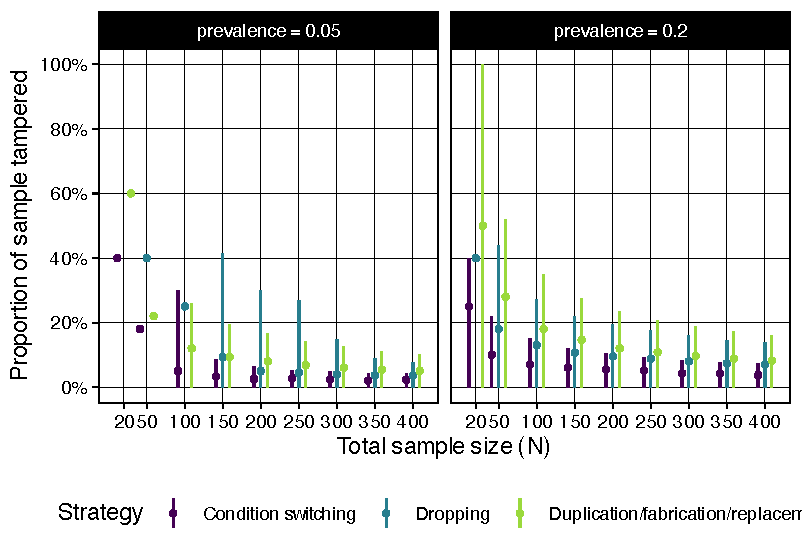
\includegraphics[width=1\linewidth,height=\textheight,keepaspectratio]{manuscript_files/figure-pdf/fig-2x2-1.pdf}

}

\caption{\label{fig-2x2}2x2 association (chi-square) setting, by outcome
prevalence: the number of tampered cells needed to first reach p
\textless{} .05 (top) and the same effort as a proportion of the sample
(bottom). Points are censoring-aware medians and bars are interquartile
ranges; a bar ending in a hollow triangle is open-ended, its upper
quartile falling among datasets that never attained significance. At
prevalence .05 and N = 20, a majority of datasets cannot be pushed to
significance at all by dropping, so even the median is not attained and
no point is drawn for it. K = 10,000 iterations per condition.}

\end{figure}%

\subsection{Effort is small, and falls as a share of the sample as
studies
grow}\label{effort-is-small-and-falls-as-a-share-of-the-sample-as-studies-grow}

Across both continuous settings the absolute number of tampered data
points needed to manufacture significance grows with sample size, but
only slowly: median counts run from 2--10 points at \(N = 20\) to 4--24
at \(N = 400\), a twentyfold increase in sample size met by roughly a
threefold increase in effort (Figure~\ref{fig-meandiff},
Figure~\ref{fig-correlation}). Expressed as a share of the sample,
effort therefore falls: from 10.0\%--50.0\% at \(N = 20\) to
1.0\%--6.0\% at \(N = 400\), a reduction of between 6.7- and 10.0-fold
depending on the strategy. Manufacturing a false positive is not merely
no harder in a large study than in a small one; proportionally it is
considerably easier. The intuition that a large sample is robust to a
few altered observations is exactly backwards. Framed as a budget: at
\(N = 400\), the proportion of datasets that would require more than
10\% of the sample to be tampered is at most 21.4\% for the least
efficient continuous-setting strategy, and for the cheapest it is 0.0\%.
Only 21.4\% of datasets resist the least effective strategy altogether
at that sample size.

The 2×2 setting is the partial exception that illustrates the mechanism
(Figure~\ref{fig-2x2}). With a rare outcome (prevalence .05) and small
samples there is simply not enough signal-bearing data to tamper with:
at \(N = 20\), 60\% of datasets cannot be pushed to significance by
dropping at all as the strategy exhausts the table's hostile cells
first. Where tampering is structurally possible, rare outcomes are cheap
to tip, because each fabricated or relabelled case moves the test
statistic disproportionately.

\subsection{The stealthiest strategies are among the
cheapest}\label{the-stealthiest-strategies-are-among-the-cheapest}

Strategies in every figure are ordered by their median proportion
tampered, computed from the data at render time. The forensically
critical result is where the label-switching family sits in that
ordering. In the two-group design, condition switching is the second
cheapest of the five strategies (median 5 switched labels at
\(N = 100\)) despite leaving every univariate distribution untouched.
Its correlation analogue, re-pairing (median 8 re-paired values at
\(N = 100\)), is not the cheapest in its setting. High-leverage
replacement and fabrication are cheaper, but it costs about the same as
unprincipled case deletion and less than duplication, while preserving
both marginal distributions exactly. Neither manipulation is detectable
by any check of a variable in isolation; only the joint structure is
disturbed. Efficiency and detectability are therefore not in tension for
the would-be fraudster: in each setting, at least one of the cheapest
strategies is also among the least visible.

\clearpage
\begin{landscape}

\begingroup\fontsize{9}{11}\selectfont

\begin{longtable}[t]{llrrrrrr}

\caption{\label{tbl-results}Tampering effort at a representative sample
size (total N = 100), by setting and strategy. Values in parentheses are
+/-1 Monte Carlo standard error. Never is the proportion of datasets for
which significance was never attained, tampering having run to a
structural limit. The two budget columns are post hoc tampering budgets:
the proportion of datasets needing more than that share of the sample
tampered, never-significant datasets exceeding every budget by
definition. The median is computed over all iterations with
never-significant ones ranked above every finite count, and is also
given as a proportion of the sample (Prop.). PI is the 95\% prediction
interval, the 2.5th-97.5th percentile of the tamper counts across
iterations; the figures show interquartile ranges instead, for the
reason given in the Methods. D/f/r denotes the duplication, fabrication
and replacement strategies, which coincide for binary data.}

\tabularnewline

\toprule
Setting & Strategy & Never & > 10\% & > 25\% & Median & 95\% PI & Prop.\\
\midrule
 & Condition switching & 0.000 (0.000) & 0.020 (0.001) & 0.000 (0.000) & 5.0 (0.0) & {}[0, 10] & 0.050 (0.000)\\
\nopagebreak
 & Dropping & 0.000 (0.000) & 0.414 (0.005) & 0.001 (0.000) & 9.0 (0.0) & {}[0, 20] & 0.090 (0.000)\\
\nopagebreak
 & Duplication & 0.000 (0.000) & 0.659 (0.005) & 0.081 (0.003) & 14.0 (0.0) & {}[0, 28] & 0.140 (0.000)\\
\nopagebreak
 & Fabrication & 0.000 (0.000) & 0.625 (0.005) & 0.001 (0.000) & 12.0 (0.6) & {}[0, 22] & 0.120 (0.006)\\
\nopagebreak
\multirow[t]{-4}{*}[\normalbaselineskip]{\raggedright\arraybackslash Mean difference} & Replacement & 0.000 (0.000) & 0.062 (0.002) & 0.000 (0.000) & 4.0 (0.0) & {}[0, 13] & 0.040 (0.000)\\
\cmidrule{1-8}\pagebreak[0]
 & Dropping & 0.000 (0.000) & 0.345 (0.005) & 0.001 (0.000) & 8.0 (0.0) & {}[0, 19] & 0.080 (0.000)\\
\nopagebreak
 & Duplication & 0.000 (0.000) & 0.638 (0.005) & 0.102 (0.003) & 13.0 (0.2) & {}[0, 32] & 0.130 (0.002)\\
\nopagebreak
 & Fabrication & 0.000 (0.000) & 0.000 (0.000) & 0.000 (0.000) & 4.0 (0.0) & {}[0, 6] & 0.040 (0.000)\\
\nopagebreak
 & Re-pairing & 0.233 (0.004) & 0.354 (0.005) & 0.233 (0.004) & 8.0 (0.0) & {}[0, never] & 0.080 (0.000)\\
\nopagebreak
\multirow[t]{-4}{*}[\normalbaselineskip]{\raggedright\arraybackslash Correlation} & Replacement & 0.000 (0.000) & 0.000 (0.000) & 0.000 (0.000) & 3.0 (0.0) & {}[0, 6] & 0.030 (0.000)\\
\cmidrule{1-8}\pagebreak[0]
 & Condition switching & 0.006 (0.001) & 0.140 (0.003) & 0.034 (0.002) & 5.0 (0.0) & {}[0, 30] & 0.050 (0.000)\\
\nopagebreak
 & Dropping & 0.057 (0.002) & 0.735 (0.004) & 0.445 (0.005) & 25.0 (0.5) & {}[0, never] & 0.250 (0.005)\\
\nopagebreak
\multirow[t]{-2}{*}[\normalbaselineskip]{\raggedright\arraybackslash 2x2, prev. 0.05} & D/f/r & 0.006 (0.001) & 0.617 (0.005) & 0.032 (0.002) & 12.0 (0.5) & {}[0, 26] & 0.120 (0.005)\\
\cmidrule{1-8}\pagebreak[0]
 & Condition switching & 0.000 (0.000) & 0.263 (0.004) & 0.000 (0.000) & 7.0 (0.0) & {}[0, 15] & 0.070 (0.000)\\
\nopagebreak
 & Dropping & 0.000 (0.000) & 0.629 (0.005) & 0.040 (0.002) & 13.0 (0.0) & {}[0, 27] & 0.130 (0.000)\\
\nopagebreak
\multirow[t]{-2}{*}[\normalbaselineskip]{\raggedright\arraybackslash 2x2, prev. 0.2} & D/f/r & 0.000 (0.000) & 0.788 (0.004) & 0.224 (0.004) & 18.0 (0.2) & {}[0, 35] & 0.180 (0.002)\\
\bottomrule

\end{longtable}

\endgroup{}

\end{landscape}
\clearpage

\section{Discussion}\label{discussion}

The distance from a null dataset to a statistically significant one is
short and cheap. The median effort is a small percentage of the sample
across strategies and settings, and for most strategies a minority of
datasets require more than 10\% of the sample to be tampered. Where
tampering fails outright it is because it is structurally impossible
rather than merely expensive. Specifically, the rare-outcome 2×2 cells,
where too few hostile cases exist to move the table at all. The share of
the sample that must be altered falls as samples grow, by roughly an
order of magnitude across the range examined, so the intuition that a
large study is protected by its size is not merely optimistic but
inverted; this extends the finding for \emph{p}-hacking that larger
samples alone do not reduce its success rate
(\citeproc{ref-stefan_big_2023}{Stefan \& Schönbrodt, 2023}). The
strategies that preserve univariate distributions (condition switching
and re-pairing) are among the most effective. Further research is
necessary to understand the relative statistical detectability of each
of these strategies.

Adding invented cases, deleting inconvenient ones, and relabelling
existing ones all require a comparable number of edits. The one clause
of the definitions that unifies them is a consequence criterion rather
than a mechanism one, such that the research is not accurately
represented in the research record, and every strategy here satisfies it
identically. Each produces a result that did not exist before.

The practical asymmetry, then, is not in the acts but in how they are
regarded. Excluding inconvenient participants is admitted by 38--43\% of
researchers and rated as close to defensible; falsifying data is
admitted by under 2\% and rated as indefensible
(\citeproc{ref-john_measuring_2012}{John et al., 2012}). When
respondents are given provable deniability, admitted fabrication and
falsification converge to indistinguishable rates
(\citeproc{ref-gopalakrishna_prevalence_2022}{Gopalakrishna et al.,
2022}) --- evidence that the gap is substantially one of reporting
rather than of behaviour. And since perceived seriousness is the
strongest available predictor of engagement
(\citeproc{ref-entradas_shades_2026}{Entradas et al., 2026}), a
seriousness ranking that is mis-set on the dimension these results
measure is not merely an intellectual inconsistency: it is a live cause
of the behaviour. Deleting a hostile case and inventing a favourable one
are, in effort and in damage to the evidence, the same act.

The ethics of reporting the results of this simulation study were given
considerable thought. Although the simulations were designed to make a
continuum visible rather than to provide a recipe, in principle, this
article documents knowledge that could be weaponised by bad actors. At
the same time, the tampering strategies simulated here have been
publicly described for years (\citeproc{ref-brown_condition_2020}{Brown,
2020}; \citeproc{ref-chambers_seven_2017}{Chambers, 2017}); what is
added here is quantification. This quantification could help change
future scientific behavior, by raising awareness around how impactful
even a very small number of data tampers can be.

The strategies employed in this simulation are deliberately simple and
greedy. Real, detection-aware fraud could plausibly trade efficiency for
plausibility. However, there are of course many cases of
detection-unaware fraud caught because of impossible or implausible
results and data, and the prevalence of undetected, relatively expert
research fraud is unknown by its very nature. Conversely, several naive
strategies here leave potentially detectable signatures (e.g., truncated
distributions after dropping; leverage outliers after fabrication;
shifted marginal prevalence in the 2×2). Future research is needed to
examine such detectability via statistical means and modern forensic
tools (\citeproc{ref-brown_grim_2017}{Brown \& Heathers, 2017};
\citeproc{ref-heathers_recovering_2018}{Heathers et al., 2018};
\citeproc{ref-wilkinson_inspect-sr_2025}{Wilkinson et al., 2025}).
However, the other distribution-preserving strategies imply that
relatively statistically invisible tampering is cheap and effective.
Auditable chain-of-custody for data, such as those employed in medical
clinical trials that allowed the the US FDA to detect abnormalities in
the trial, as discussed in the introduction, would be needed to prevent
or detect such forms of tampering
(\citeproc{ref-us_food_and_drug_administration_center_for_drug_evaluation_and_research_proposal_2026}{U.S.
Food and Drug Administration, Center for Drug Evaluation and Research,
2026}). Infrastructure for auditable chain-of-custody is rare in other
fields.

\section*{Data and code availability}\label{data-and-code-availability}
\addcontentsline{toc}{section}{Data and code availability}

All simulation code and results, including extended ADEMP
specifications, per-condition tables, and Monte Carlo standard errors
for every estimate, are available at
\url{https://github.com/ianhussey/simulation-impact-of-data-tampering}.

\section*{References}\label{references}
\addcontentsline{toc}{section}{References}

\phantomsection\label{refs}
\begin{CSLReferences}{1}{0}
\bibitem[\citeproctext]{ref-brown_condition_2020}
Brown, N. J. L. (2020). \emph{{In his excellent book {``The 7 Deadly
Sins of Psychology,''} @chrisdc77 provides a list of 12 tips for people
who want to get away with scientific fraud. Let's skip the question of
where he acquired that expertise and look at just one tip: Swap
participants between conditions. /1}}.
\url{https://x.com/sTeamTraen/status/1329203865649094656}

\bibitem[\citeproctext]{ref-brown_grim_2017}
Brown, N. J. L., \& Heathers, J. A. J. (2017). The {GRIM} {Test}: {A}
{Simple} {Technique} {Detects} {Numerous} {Anomalies} in the {Reporting}
of {Results} in {Psychology}. \emph{Social Psychological and Personality
Science}, \emph{8}(4), 363--369.
\url{https://doi.org/10.1177/1948550616673876}

\bibitem[\citeproctext]{ref-chambers_seven_2017}
Chambers, C. (2017). \emph{The seven deadly sins of psychology: {A}
manifesto for reforming the culture of scientific practice}. Princeton
University Press. \url{https://doi.org/10.1515/9781400884940}

\bibitem[\citeproctext]{ref-entradas_shades_2026}
Entradas, M., Feng, Y., \& Sousa, I. C. e. (2026). The '{shades} of
grey' in research integrity---{Researchers} admit to questionable
research practices that they do not perceive to be serious. \emph{PLOS
ONE}, \emph{21}(1), e0339056.
\url{https://doi.org/10.1371/journal.pone.0339056}

\bibitem[\citeproctext]{ref-fanelli_how_2009}
Fanelli, D. (2009). How many scientists fabricate and falsify research?
{A} systematic review and meta-analysis of survey data. \emph{PLoS ONE},
\emph{4}(5), e5738. \url{https://doi.org/10.1371/journal.pone.0005738}

\bibitem[\citeproctext]{ref-gopalakrishna_prevalence_2022}
Gopalakrishna, G., Riet, G. ter, Vink, G., Stoop, I., Wicherts, J. M.,
\& Bouter, L. M. (2022). Prevalence of questionable research practices,
research misconduct and their potential explanatory factors: {A} survey
among academic researchers in {The} {Netherlands}. \emph{PLOS ONE},
\emph{17}(2), e0263023.
\url{https://doi.org/10.1371/journal.pone.0263023}

\bibitem[\citeproctext]{ref-heathers_recovering_2018}
Heathers, J. A. J., Anaya, J., Zee, T. van der, \& Brown, N. J. L.
(2018). \emph{Recovering data from summary statistics: {Sample}
{Parameter} {Reconstruction} via {Iterative} {TEchniques} ({SPRITE})}.
PeerJ Preprints. \url{https://doi.org/10.7287/peerj.preprints.26968v1}

\bibitem[\citeproctext]{ref-john_measuring_2012}
John, L. K., Loewenstein, G., \& Prelec, D. (2012). Measuring the
prevalence of questionable research practices with incentives for truth
telling. \emph{Psychological Science}, \emph{23}(5), 524--532.
\url{https://doi.org/10.1177/0956797611430953}

\bibitem[\citeproctext]{ref-morris_using_2019}
Morris, T. P., White, I. R., \& Crowther, M. J. (2019). Using simulation
studies to evaluate statistical methods. \emph{Statistics in Medicine},
\emph{38}(11), 2074--2102. \url{https://doi.org/10.1002/sim.8086}

\bibitem[\citeproctext]{ref-schiller_addendum_2018}
Schiller, D., Monfils, M.-H., Raio, C. M., Johnson, D. C., LeDoux, J.
E., \& Phelps, E. A. (2018). Addendum: {Preventing} the return of fear
in humans using reconsolidation update mechanisms. \emph{Nature},
\emph{562}(7727), E21--E21.
\url{https://doi.org/10.1038/s41586-018-0405-7}

\bibitem[\citeproctext]{ref-siepe_simulation_2024}
Siepe, B. S., Bartoš, F., Morris, T. P., Boulesteix, A.-L., Heck, D. W.,
\& Pawel, S. (2024). Simulation studies for methodological research in
psychology: {A} standardized template for planning, preregistration, and
reporting. \emph{Psychological Methods}.
\url{https://doi.org/10.1037/met0000695}

\bibitem[\citeproctext]{ref-spiess_scientific_2024}
Spiess, A.-N., Rödiger, S., Schaks, M., Burdukiewicz, M., \&
Tellinghuisen, J. (2024). \emph{Scientific reasoning driven by
influential data: Resuscitate dfstat!} bioRxiv.
\url{https://doi.org/10.1101/2024.10.30.621016}

\bibitem[\citeproctext]{ref-stefan_big_2023}
Stefan, A. M., \& Schönbrodt, F. D. (2023). Big little lies: A
compendium and simulation of p-hacking strategies. \emph{Royal Society
Open Science}, \emph{10}(2), 220346.
\url{https://doi.org/10.1098/rsos.220346}

\bibitem[\citeproctext]{ref-steneck_introduction_2007}
Steneck, N. H. (2007). \emph{Introduction to the {Responsible} {Conduct}
of {Research}}. \url{https://doi.org/10.1037/e638422011-001}

\bibitem[\citeproctext]{ref-us_food_and_drug_administration_center_for_drug_evaluation_and_research_proposal_2026}
U.S. Food and Drug Administration, Center for Drug Evaluation and
Research. (2026). \emph{Proposal to {Withdraw} {Marketing} {Approval};
{Notice} of {Opportunity} for a {Hearing}: {TAVNEOS} (avacopan) capsule,
10 mg, {NDA} 214487} (Letter to \{Amgen\}, \{Inc\}. Docket No.
FDA-2026-N-1321). U.S. Food; Drug Administration.
\url{https://www.fda.gov/media/192160/download}

\bibitem[\citeproctext]{ref-verfaellie_case_2011}
Verfaellie, M., \& McGwin, J. (2011). The case of {Diederik} {Stapel}.
\emph{APA Psychological Science Agenda}.
\url{https://www.apa.org/science/about/psa/2011/12/diederik-stapel}

\bibitem[\citeproctext]{ref-wang_researcher_2018}
Wang, M. Q., Yan, A. F., \& Katz, R. V. (2018). Researcher {Requests}
for {Inappropriate} {Analysis} and {Reporting}: {A} {U}.{S}. {Survey} of
{Consulting} {Biostatisticians}. \emph{Annals of Internal Medicine},
\emph{169}(8), 554--558. \url{https://doi.org/10.7326/M18-1230}

\bibitem[\citeproctext]{ref-wilkinson_inspect-sr_2025}
Wilkinson, J., Heal, C., Flemyng, E., Antoniou, G. A., Aburrow, T.,
Alfirevic, Z., Avenell, A., Barbour, V., Berghella, V., Bishop, D. V.
M., Bordewijk, E. M., Brown, N. J. L., Christopher, J., Clarke, M.,
Dahly, D., Dennis, J., Dicker, P., Dumville, J., Frankish, H., \ldots{}
Kirkham, J. J. (2025). \emph{{INSPECT}-{SR}: A tool for assessing
trustworthiness of randomised controlled trials}. medRxiv.
\url{https://doi.org/10.1101/2025.09.03.25334905}

\bibitem[\citeproctext]{ref-xie_prevalence_2021}
Xie, Y., Wang, K., \& Kong, Y. (2021). Prevalence of {Research}
{Misconduct} and {Questionable} {Research} {Practices}: {A} {Systematic}
{Review} and {Meta}-{Analysis}. \emph{Science and Engineering Ethics},
\emph{27}(4), 41. \url{https://doi.org/10.1007/s11948-021-00314-9}

\end{CSLReferences}




\end{document}
